% !TEX root =  master.tex
\cleardoublepage
\chapter{Grundlagen des PCR-Poolings}
In diesem Kapitel sollten Methoden für das PCR-Pooling beschrieben werden.
Begonnen wird mit einem einfachen, eindimensionalen Poolingverfahren als spätere Referenz.
Kompliziertere Verfahren werden später erläutert um zu prüfen, ob hierdurch ein Mehrwert beobachtet werden kann.
Hierdurch wird sichergestellt, dass das einfachstmögliche Verfahren angewandt wird.
Umfangreiche Methoden werden nur weiter verfolgt, wenn sie das einfache Referenzverfahren übertreffen.

\section{Eindimensionales Pooling}
Das einfachste Verfahren für Pooling ist, eine eindimensionale Reihe von Proben zu verwenden und diese vor der PCR-Analyse zu kombinieren.
Die Matrix lässt sich hierbei als 1xN beschreiben.
Die Proben werden gemeinsam getestet.
\begin{itemize}
	\item \textbf{Negatives Poolergebnis:}\newline
	Ein negatives Gesamtergebnis bedeutet, dass \textbf{jede Einzelprobe negativ} war.
	
	Es wurde somit durch einen Test festgestellt, dass alle Personen im Pool negativ sind.
	
	Die Effizienz lässt sich somit beschreiben als $\frac{Anzahl Testpersonen (N)}{Anzahl Tests (1)} $.
	
	\item \textbf{Positives Poolergebnis:}\newline
	Ein positives Gesamtergebnis bedeutet, dass \textbf{mindestens eine Einzelprobe positiv} war.
	
	In diesem Fall müssen weitere Tests durcheführt werden, um die positiven Einzelpersonen zu ermitteln.
	Die Tests erfolgen hierbei nacheinander und sind statistisch unabhängig voneinander.
	
	Die Nachtestung kann durch mehrstufiges Pooling optimiert werden.
	Für das einfachste Basisverfahren wird allerdings angenommen, dass nach einem Positivergebnis das Pooling beendet wird.
	Die Personen innerhalb des positiven Pools werden einzeln nachgetestet.\footnote{Viehweger Zeile 11}
	
	Im Falle einer Nachtestung wird somit ein initialer Test für den Pool benötigt, welcher positiv ausfällt.
	Danach werden nochmal Tests für jede Einzelperson benötigt.
	
	Die Effizienz lässt sich somit beschreiben als $\frac{Anzahl Testpersonen (N)}{1 Pooltest + N Einzeltests} $.
\end{itemize}


Die Testung erfolgt zweistufig.

Der Erwartungswert für die benötigte Anzahl der Tests lässt sich beschreiben als:

Wenn(Pool Positiv)
Dann -> N+1
Andernfalls -> 1

Der erwartete Testbedarf hängt ab von der Wahrscheinlichkeit, dass der Pool positiv ist.
Dieser lässt sich durch die prozentuale Angabe der Testprävalent ermitteln.

Hieraus ergibt sich:
%Erwartungswert Testbedarf = (P(Positiv) * N+1) + (!P(Positiv) * 1)
%N/((MIN(1;N*Prävalenz)*(N+1))+(1-MIN(1;N*Prävalenz)))

P(PoolPositiv) = $(min\left(1;Poolsize\cdot Pravalenz\right)$

Erwartungswert Personen pro Test =
$\frac{Poolsize}{P(PoolPositiv)\cdot (Poolsize + 1)) + (1 - P(PoolPositiv))}$

Der Erwartungswert ist also abhängig von zwei Variablen: Der Prävalenz, welche zur Positivwahrscheinlichkeit des Pools führt, und der Testgröße, welche frei gewählt werden kann.

Für jeden gegebene Testgröße lässt sich der Erwartungswert als abhängige Variable der Prävalenz darstellen.

Unterschiedliche Testgrößen bilden hierbei unterschiedliche Kurvenverläufe.
Allerdings muss nicht für den gesamten Prävalenzspektrum derselbe Test zum einsatz kommen.

Für jede Prävalenz kann somit errechnet werden, welche Testgröße den optimalen Erwartungswert ergibt.

Einen Effizienzwechsel findet man immer an den Schnittpunkten der Effizienzkurven.



\cleardoublepage
\subsubsection{Effizienzkurve Eindimensionale Pools}
Für das eindimensionale Poolingverfahren ergibt sich insgesamt die folgende Effizienzkurve.

Eine vollständige gegenüberstellung in tabellarischer Form ist im Anhang dargestellt.
\begin{figure}[h]
	\centering
	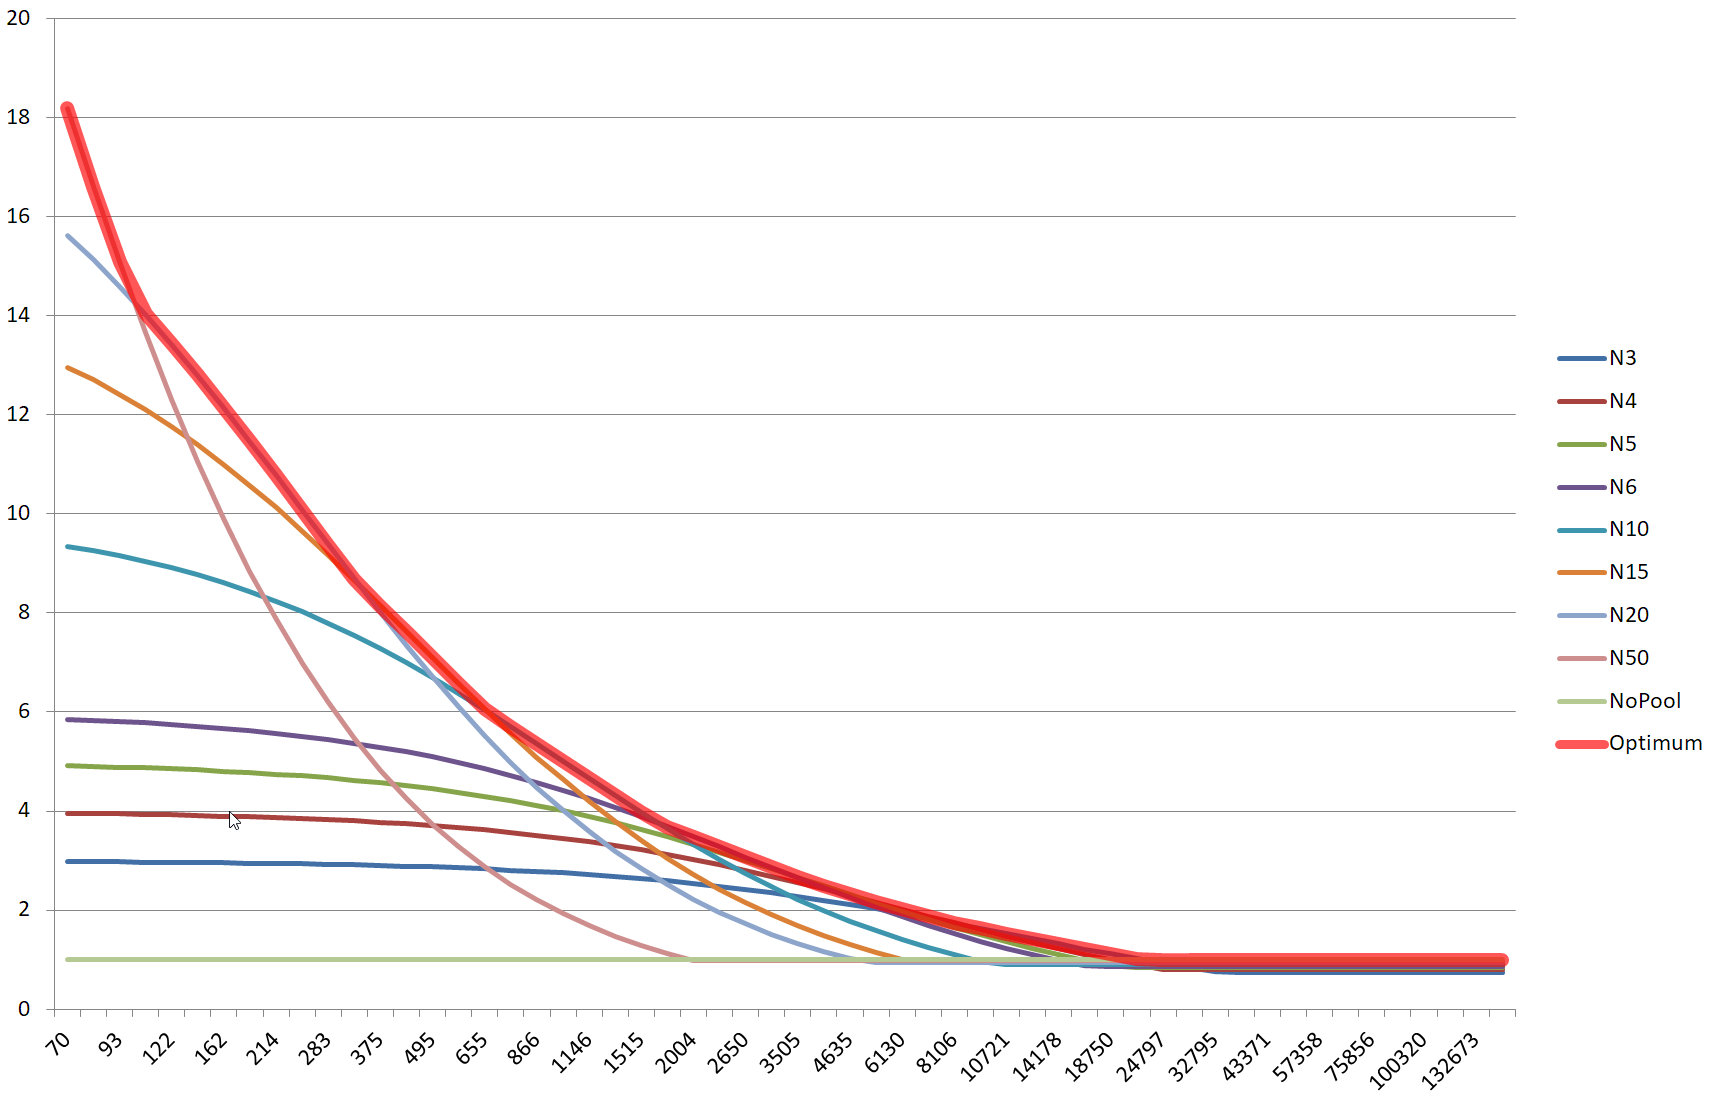
\includegraphics[height=.6\textwidth]{img/1D_Pool-EffKurve}
	\caption{Effizienzkurve des eindimensionalen Poolingverfahrens\footnotemark}
\end{figure}

Als logarithmische Tabelle bedeutet dies:

\begin{tabular}{|c|c|}
	\hline
	Prävalenz (von 100.000) & Erwartungswert \\
	\hline
	1 & sdf \\
	\hline
	10 & sdf \\
	\hline
	100 & asdad \\
	\hline
	1.000 & sdfsd \\
	\hline
	10.000 & dfg \\
	\hline
	100.000 & dfg \\
	\hline
\end{tabular}

\cleardoublepage
\section{Zweidimensionales Pooling}
Bei dieser Poolingmethode handelt es sich um einen zweidimensionalen Pool, mit dem Ziel, den Bedarf einer Nachtestung bei einzelnen Positivfällen zu minimieren.
Die Testpersonen werden in einer AxB-Matrix angeordnet.
Die Proben werden dann für jede Spalte und jede Reihe gepoolt.
Allgemein formuliert lässt sich sagen:
Testbedarf pro Person =
$\frac{A+B}{A\cdot B}$

Die Testgruppe lässt sich geometrisch als Rechteck beschreiben.
Die Kanten A und B ergeben in Summe die benötigte Testanzahl.
Die Fläche beschreibt die mögliche Anzahl der zu testenden Personen.
Aus der Geometrie ist bekannt,\footnote{Geometrie Quadrat}
dass das Verhältnis von Fläche zu Kantenlänge bei einem Quadrat optimal ist.
Bei dieser Methode kommen somit nur Quardate als effizient infrage.
Hierdurch lässt sich festlegen, dass $A=B$.

Für eine Testgruppe von 25 Personen, welche in einer 5x5 Matrix angeordnet sind, werden somit 5+5 Tests benötigt.
Die Effizienz läge bei 2,5 Personen pro Test.
Vergleichen mit dem eindimensionalen Poolingverfahren klingt das zunächst nicht nach sehr viel.
Allerdings ist dieses Verfahren darauf optimiert, robust gegen einzelne Positivfälle zu sein.
Die Hypothese wäre somit, dass es bei hohen Prävalenzen einen Vorteil bietet, da nicht alle Testpersonen erneut getestet werden müssen.

Die Wahrscheinlichkeit, dass der Pool positiv ist verändert sich zum anderen Testverfahren nicht.
Sie hängt wieder von Prävalenz und Größe der Testgruppe ab.
Deshalb gilt weiterhin:
P(PoolPositiv) = $(min\left(1;Poolsize\cdot Pravalenz\right)$

Bei der Nachtestung im Falle eines positiven Pools werden allerdings nicht mehr alle Personen nachgetestet.
Sollte nur eine Person in der Testgruppe positiv sein, so kann dessen Position in der Testgruppe anhand der positiven Pools abgelesen werden.
\begin{figure}[h]
	\centering
	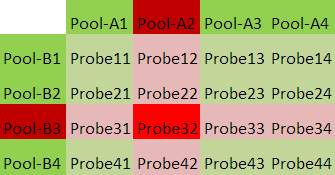
\includegraphics[height=.25\textwidth]{img/2d_Pool_1Positiv}
	\caption{Zweidimensionaler Pool mit einer positiven Person (Probe32). Die Pools A2 und B3 werden positiv und weisen auf die Position 3-2 der positiven Probe. Für die Hellrot unterlegten Personen liegt ein positiver und ein Negativer Pool vor.\footnotemark}
\end{figure}

Erwartungswert Personen pro Test =
%$\frac{A\cdot A} {P(PoolPositiv)\cdot (Poolsize + 1)) + (1 - P(PoolPositiv))}$

\subsubsection{Sicherheitsniveaus}

An dieser Stelle ist zu bemerken, dass es innerhalb der Testgruppe drei Kategorien von Testergebnis gibt.
\begin{itemize}
	\item \textbf{2x Positiv} Bei Probe 3-2 (rot) sind als einziges beide Pooltests A2 und B3 positiv ausgefallen. Diese Person ist höchstwahrscheinlich positiv und wird einzeln nachgetestet.
	\item \textbf{1x Positiv} 6 Proben (hellrot) weisen ein positives und ein negatives Ergebnis auf.
	\item \textbf{beide negativ} Bei den verbleibenden Personen (grün) sind zwei unabhängige Pooltests negativ. Sie sind höchstwahrscheinlich nicht infiziert.
\end{itemize}
Hieraus ergibt sich nun die Frage, welcher Sicherheitsanspruch gegenüber dem Test erhoben wird.
Eine Person mit zwei positiven Testergebnissen ist höchstwahrscheinlich infiziert und wird in jedem Fall einzeln nachgetestet.
Eine Person mit zwei negativen Testergebnisen ist höchstwahrscheinlich nicht infiziert und bekommt ein negatives Testzertifikat.
Wie sollte man nun mit den Personen verfahren, die Teil eines positiven Pools waren?

\begin{itemize}
	\item \textbf{Hohes Sicherheitsniveau} Alle zweifelhaften Personen werden einzeln nachgetestet.
	\item \textbf{Mittleres Sicherheitsniveau} Alle zweifelhaften Personen werden in einen eindimensionalen Pool kombiniert und gemeinsam getestet. Hierdurch kann ermittelt werden, ob beim ersten Durchlauf Fehler passiert sind und Personen übersehen wurden. Im Falle eines Positiven Poolergebnisses müssen alle einzeln nachgetestet werden. Hierduch werden drei sequenzielle Durchläufe notwendig, was die Übermittlung des Testergebnisses inakzeptabel lang verzögern kann.
	\item \textbf{Geringes Sicherheitsniveau} Die Personen für welche es keine Überschneidung gibt, werden als negativ gewertet. In einer perfekten Modellwelt mit 100 Prozent genauen Tests und keinen Anwendungsfehlern wäre auch dies unproblematisch. In der Realität können hierdurch aber falsch-negative Ergebnisse übermittelt werden.
\end{itemize}

\subsubsection{Mehrere Positivfälle}

Schwieriger wird es zudem, wenn mehrere Personen innerhalb des Pools positiv sind.
Die Positiven Tests lassen sich dann nicht mehr exakt einer Person zuordnen.
Die beiden positiven Personen (1-4 und 3-2) in Abb 3.3 lösen die Tests A2, A4, B1 und B3 aus.
Neben den positiven Personen zeigen diese Tests auch auf die eigentlich negativen Proben 1-2 und 3-4.
Aus diesem Grund müssen hier für zwei positive Personen vier Proben nachgetestet werden.

\begin{figure}[h]
	\centering
	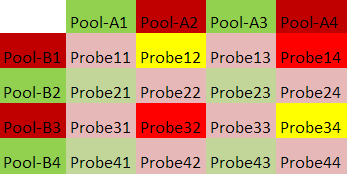
\includegraphics[height=.25\textwidth]{img/2d_Pool_2Positiv}
	\caption{Zweidimensionaler Pool mit zwei positiven Personen (rot). Es treten zwei False-Positives auf (gelb).\footnotemark}
\end{figure}

Grundsätzlich verhält sich der Bedarf an Nachtestungen quadratisch zur Anzahl der Positiven Personen.
Es ist allerdings möglich, dass mehrere positive Personen in einem Test sind.
Durch diese Überschneidung verringert sich der Bedarf für Nachtestungen, weswegen eine Clusterung positiver Tests vorteilhaft sein kann.


\cleardoublepage
